\documentclass{article}
\usepackage{amsthm}
\usepackage{amssymb}
\usepackage{pgf, tikz}
\usetikzlibrary{arrows, automata}
\begin{document}
\title{Homework 10}
\author{Will Boland}
\maketitle

\textbf{Question 1}\newline
A) i) No, (c, c) $\notin$ R\newline
ii) No, (a, a) $\in$ R\newline
iii) No, (a, b) $\in$ R, but (b, a) $\notin$ R\newline
iv) Yes, every instance of (x, y) and (y, x) that is reflexive in R, it has x = y\newline
v) Yes, everytime you have (x, y) and (y, z) in R, you have (x, z) \newline\newline

B) i) Yes, it includes all the required pairs (1,1), (2, 2), and (3, 3)\newline
ii) No, (1, 1) $\in$ S\newline
iii) No, (3, 2) $\notin$ S\newline
iv) No, R(1, 2) and R(2, 1) but 1 $\neq$ 2\newline
v) No, S(1, 2) and S(2, 4) but (1, 4) $\notin$ S\newline\newline

C) i) Yes, for any x $\in$$\mathbb{Z}$E, x + x is even, so E(x, x)\newline
ii) No, for any x $\in$ $\mathbb{Z}$, x + x is even, so E(x, x)\newline
iii) Yes, for any x $\in$ $\mathbb{Z}$, where x + y is even, so is y + x, so E(x, y) and E(y, x)\newline
iv) No, for any x $\in$ $\mathbb{Z}$, where x + y is even, so is y + x, so E(x, y) and E(y, x)\newline
v) Yes, for any x $\in$ $\mathbb{Z}$, where x + y is even, and y + z is even, there exists an x + z that is also even\newline\newline
 
D) i) No, because ("ABC", "ABC") $\notin$ C\newline
ii) Yes, because no instance of members of C are of (x, x) for any substring due to $s$ being a proper substring of $t$\newline
iii) No, ("ABC", "ABCD") $\in$ C but ("ABCD", "ABC") $\notin$ C\newline
iv) Yes, but only trivially as there are no instances where (x, y) $\in$ C and (y, x) $\in$ C.\newline
v) Yes, because every (x, y) and (y, z) has a (x, z) due to y being based off of z and x being based off of x.\newline\newline

E) i) No, because for it to intersect it has to have members that are the same which conflict the requirement\newline
ii) Yes, because (x, x) $\notin$ D because the intersection would not just be the empty set\newline
iii) Yes becuase the order of sets doesn't matter for the intersection\newline
iv) No because The intersection will be the empty set, so no two sets will be the same \newline
v) Yes, because if D(x, y) then X and y dont intersect other than the empty set meaning D(y, z) that y and z dont intersect so D(x, z).\newline\newline

\textbf{Question 2}\newline
A) The relation X = \{(a, d), (d, a)\}\newline
B) The relation R = \{(2, 1), (2, 2), (1, 3), (3, 3)\}\newline
C) The relation T = \{(2, 4), (4, -6), (2, -6)\}\newline
D) \newline
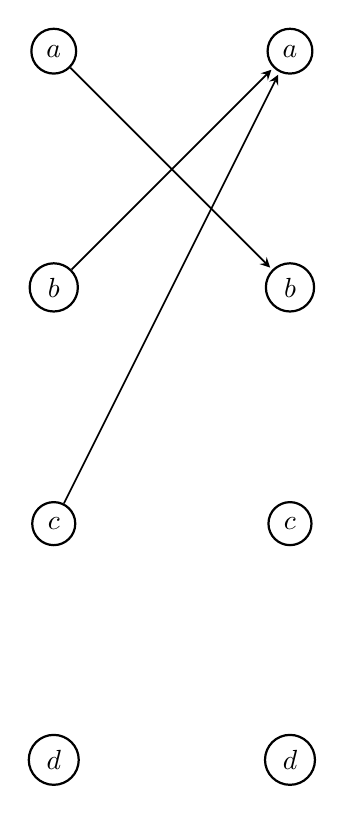
\begin{tikzpicture}[
            > = stealth, % arrow head style
            shorten > = 1pt, % don't touch arrow head to node
            auto,
            node distance = 3cm, % distance between nodes
            semithick % line style
        ]

        \tikzstyle{every state}=[
            draw = black,
            thick,
            fill = white,
            minimum size = 4mm
        ]

	\node[state] (a) {$a$};
	\node[state] (b) [below of=a] {$b$};
	\node[state] (c) [below of=b] {$c$};
	\node[state] (d) [below of=c] {$d$};
	\node[state] (aa) [right of=a] {$a$};
	\node[state] (bb) [below of=aa] {$b$};
	\node[state] (cc) [below of=bb] {$c$};
	\node[state] (dd) [below of=cc] {$d$};
	
        \path[->] (a) edge node {} (bb);
        \path[->] (b) edge node {} (aa);
        \path[->] (c) edge node {} (aa);

    \end{tikzpicture}\newline
E) Cannot exist because there are a finite set of english words\newline\newline
F) The relation F = \{(x, y) $\mid$ where x = ${2}^y$ $\wedge$ y $\neq$ x\}\newline
G) The relation P = \{(Will Boland, Will Boland), (Will Boland, Will Boland)\} where "Will Boland" is the same person.\newline
H) The relation (L) cannot exist because if it is anti-symmetric then L(x, y) and L(y, x) and x = y but if it is anti-reflexive x $\neq$ y\newline
I) The relation S = \{(Will Boland, Will Boland), (Will Boland, Augie), (Will Boland, Jack), (Augie, Jack), (Augie, Augie), (Jack, Jack)\}\newline\newline

\textbf{Question 3}\newline
A) \textit{Proof}\newline
Choose an integer n, and m, where m = n\newline
n = m * k where k is some integer\newline
So, m = n * k\newline
Since n = m and m$\mid$n then D(n, n)$\square$\newline

B) \textit{Proof}\newline
Choose numbers m and n and assume D(m, n) and D(n, m)\newline
That means n is divisble by m and m is divisble by n\newline
So there exists a k where n = m * k and m = n * k\newline
thus n = (n * k) * k\newline
K must be 1 otherwise n would not be divisble by m and vice versa $\square$\newline

C) $\textit{Proof}$\newline
Choose  any number m, n, and z and assume D(m, n), D(n, z)\newline
So, n is divisble by m and z is divisble by n.\newline
Thus there exists a number k where n = m * k and z = n * k\newline
So, m = n/k\newline
So, z = (n/k)*k\newline
So, z = m * k\newline
So, D(m, z)$\square$\newline\newline

\textbf{Question 4}\newline
A) \textit{Proof}\newline
Have any number x and y where 5 $\mid$ (x-y) and x = y\newline
So, (x-y) is divisble by 5\newline
So, (x-x) is divisible by 5\newline
So, $\equiv$(x, x)$\square$\newline

B) \textit{Proof}\newline
Have any number x and y and assume $\equiv$(x, y)\newline
So, (x-y) is divisble by 5\newline
So, there exists a k such that x - y = 5 * k\newline
y - x = -(x - y) = -5k = -5 * -(x - y)\newline
So therefore y - x is divisble by 5\newline
So, $\equiv$(x, y) and $\equiv$(y, x)$\square$\newline

C) \textit{Proof}\newline
Have any number x and y and z and assume $\equiv$(x, y) and $\equiv$(y, z)\newline
So x - y is divisble by 5 and y - z is divisible by 5\newline
Thus there exists a k  and j such that x - y = 5 * k and y - z = 5 * j\newline
so (x - y) + (y - z) = 5k + 5j\newline
So x - z = = 5k + 5j\newline
So, x - z = 5(k + j)\newline
since k and j are integers so is k + j\newline
Therefore x - z is divisble by 5, meaning $\equiv$(x, z)$\square$\newline




\enddocument
